\section{Proposed SCL Framework}\label{sec:method}

\scl{} is a lightweight, rule-based layer operating between a frozen detector and tracker (the
host) without modifying their underlying algorithms. Figure~\ref{fig:arch} illustrates the five
processing steps of \scl{} for frame $t$. First, Otsu-based logit partitioning (Step~1) divides
recent detection scores into background, uncertain, and confident groups. Next, detection stream
classification (Step~2) determines whether the score distribution is clean or noisy based on
historical confidence statistics. Mode-adaptive candidate selection (Step~3) then retains,
removes, or remaps detection scores and adjusts the tracker's confidence thresholds according to
the operating mode. Track-guided weak detection recovery (Step~4) allows eligible low-confidence
detections to support track continuity. Finally, camera motion-adaptive matching tolerance
(Step~5) adjusts the association criterion according to estimated camera motion. The host
contract provides the tracker's published parameters, while the tracker performs its original
association and track-management operations unchanged.

Table~\ref{tab:symbols} lists every symbol of this section in plain words, with its value in a
real example, the clean stream of Fig.~\ref{fig:groups}a; the subsections below use the same
example, so each number can be followed from the input to the output.

\begin{table}[!tb]
\caption{The symbols of Sect.~\ref{sec:method} in plain words. Example: the value in the clean
stream of Fig.~\ref{fig:groups}a (MOT17-02, frame 101, ByteTrack in its official setting), as
recorded by the frozen \scl{}; values marked e.g.\ are worked examples from the text.}
\label{tab:symbols}
\centering\footnotesize
\setlength{\tabcolsep}{3pt}
\begin{tabular}{@{}l>{\raggedright\arraybackslash}p{37mm}>{\raggedright\arraybackslash}p{22mm}@{}}
\toprule
Symbol & Meaning & Example\\
\midrule
$s_i$ & detector score of candidate $i$, between 0 and 1 & e.g.\ 0.9\\
$z_i$ & its logit, $\log\bigl(s_i/(1-s_i)\bigr)$, Eq.~\eqref{eq:logit} & e.g.\ $\log 9=2.2$\\
$W$ & number of past frames whose logits are pooled & 10\\
$Z_t^W$ & the logits of frames $t-W$ to $t-1$ & 916 logits\\
$t_1$ & first split: background lies below it & $-0.78$ (score 0.32)\\
$t_2$ & second split: confident lies above it & 0.95 (score 0.72)\\
$\rho_t$ & share of confident candidates in the foreground, Eq.~\eqref{eq:rho} & $175/263=0.67$\\
median $\rho$ & median of $\rho$ over the stream so far; clean if $\ge0.5$ & 0.63: clean\\
$a$, $b$ & the tracker's published scores to match a track and to start one & 0.6, 0.7\\
$\ell$ & the lowest score the tracker uses & 0.1\\
$m_0$ & the tracker's matching tolerance: 1 minus the smallest IoU that matches & 0.8 (IoU $\ge0.2$)\\
$a_t$, $b_t$ & the thresholds \scl{} passes for frame $t$ & 0.6, 0.7 (kept)\\
$u_i$, $\tilde{s}_i$ & rank of $s_i$ among stored scores, and the new score of the noisy mode, Eq.~\eqref{eq:remap} & e.g.\ $u_i=0.8\to\tilde{s}_i=0.9$\\
$\mathcal{T}_{t-1}$ & the tracks of the previous frame & --\\
$K_t$ & the candidates passed to the tracker & --\\
$g_t$, $r_t$ & camera shift between two frames; its ratio to the usual shift & e.g.\ $r_t=2$\\
$m_t$ & the tolerance \scl{} passes for frame $t$, Eq.~\eqref{eq:motion} & 0.8 (clean)\\
\bottomrule
\end{tabular}
\end{table}



\subsection{Inputs and outputs of SCL}\label{sec:problem}
In each frame $t$, the detector gives candidates $D_t=\{(\mathbf{x}_i,s_i,c_i)\}$, each with a box
$\mathbf{x}_i$, a score $s_i\in(0,1)$, and a class $c_i$. The layer works on the logit
\begin{equation}
z_i=\log\frac{s_i}{1-s_i},
\label{eq:logit}
\end{equation}
the log-odds transformation of the confidence score. It maps a score between 0 and 1 to an
unbounded scale and keeps the order of the scores: a score of 0.5 gives $z_i=\log1=0$, 0.9 gives
$\log(0.9/0.1)=\log9=2.2$, and 0.1 gives $\log(1/9)=-2.2$. The logistic function $\sigma(z)=1/(1+e^{-z})$ turns a logit back into a
score. The layer uses logits for two reasons. Detector scores crowd near 0 and 1, where small
differences in score are large differences in confidence; the logit spreads these regions out, so
the splits of Step~1 separate the groups more clearly. And a common change of a detector's scores,
a change of temperature, divides all logits by the same number; the splits follow this stretch,
and each group keeps the same candidates. The host gives its contract $h=(a,b,\ell,m_0)$: the score $a$ needed to match a track, the
score $b$ needed to start one, the lowest score $\ell$ it uses, and its matching tolerance $m_0$,
one minus the smallest intersection over union (IoU) of two boxes that counts as a match. A
single-stage tracker has $\ell=\min(a,b)$, a two-stage tracker $\ell<\min(a,b)$. Table~\ref{tab:contracts}
(Sect.~\ref{sec:contract}) gives these four values for every tracker and the published settings they
come from; for ByteTrack in its official setting they are $a=0.6$, $b=0.7$, $\ell=0.1$, and
$m_0=0.8$. In every frame
the layer returns
\begin{equation}
\left(K_t,\tilde{s},a_t,b_t,m_t\right)=
\mathcal{L}\left(Z_{<t},D_t,\mathcal{T}_{t-1},g_t;\,h\right):
\label{eq:layer}
\end{equation}
the candidates $K_t$ for the tracker, their scores, and its thresholds and tolerance (the arrows
into the tracker in Fig.~\ref{fig:arch}), from the logits $Z_{<t}$ of earlier frames, the tracks
$\mathcal{T}_{t-1}$, and the camera motion $g_t$ between the frames $I_{t-1}$ and $I_t$; no future
frame is used.

\begin{table*}[!t]
\caption{Host contracts: the four published settings of each tracker that \scl{} reads, and where
each value comes from. $a$: the score a detection needs to be matched to a track; $b$: the score it
needs to start a new track; $\ell$: the lowest score the tracker uses at all; $m_0$: the matching
tolerance, one minus the smallest overlap (IoU) that counts as a match. A tracker with a second
step for low scores (two-stage) has $\ell<\min(a,b)$; a tracker without it (single-stage) has
$\ell=\min(a,b)$. ByteTrack-type trackers publish $m_0$ directly (match\_thresh); SORT-type
trackers publish the IoU threshold $\theta$, and $m_0=1-\theta$.}
\label{tab:contracts}
\centering\footnotesize
\setlength{\tabcolsep}{4pt}
\begin{tabular}{@{}>{\raggedright\arraybackslash}p{30mm}lcccc>{\raggedright\arraybackslash}p{78mm}@{}}
\toprule
Tracker (setting) & Type & $a$ & $b$ & $\ell$ & $m_0$ & Published settings behind the values\\
\midrule
ByteTrack (official MOT17) & two-stage & 0.6 & 0.7 & 0.1 & 0.8 & track\_thresh 0.6; new tracks need track\_thresh $+$ 0.1; second step from 0.1; match\_thresh 0.8\\
ByteTrack (library default) & two-stage & 0.25 & 0.25 & 0.1 & 0.8 & Ultralytics bytetrack.yaml: track\_high\_thresh 0.25, new\_track\_thresh 0.25, track\_low\_thresh 0.1, match\_thresh 0.8\\
BoT-SORT (library default) & two-stage & 0.25 & 0.25 & 0.1 & 0.8 & Ultralytics botsort.yaml: the same four values\\
SparseTrack & two-stage & 0.6 & 0.7 & 0.1 & 0.85 & track\_thresh 0.6; new tracks need track\_thresh $+$ 0.1; second step from 0.1; match\_thresh 0.85\\
BoostTrack & two-stage & 0.6 & 0.6 & 0.1 & 0.7 & det\_thresh 0.6; every emitted detection (from 0.1) can be boosted; IoU threshold 0.3\\
Hybrid-SORT & two-stage & 0.6 & 0.6 & 0.1 & 0.75 & det\_thresh 0.6; low-score step from 0.1; IoU threshold 0.25\\
OC-SORT & single-stage & 0.6 & 0.6 & 0.6 & 0.7 & det\_thresh 0.6, no low-score step; IoU threshold 0.3\\
PD-SORT & single-stage & 0.6 & 0.6 & 0.6 & 0.7 & det\_thresh 0.6, no low-score step; IoU threshold 0.3\\
\bottomrule
\end{tabular}
\end{table*}


\subsection{Otsu-Based Logit Partitioning and Confidence Estimation}\label{sec:calib}
\emph{Step 1 in Fig.~\ref{fig:arch}. Input:} the logits $Z_t^W$ of the candidates of the last $W=10$ frames. \emph{Output:} the
splits $t_1$, $t_2$ and the confident share $\rho_t$.

The logits are split twice with Otsu's method \cite{otsu1979}, which picks, from the data alone
and without labels or tuning, the threshold that best separates a set of values into two groups;
applied twice, it gives the three groups that one threshold cannot. The first split, $t_1$,
separates background (low logits) from foreground; the second, $t_2$, found on the foreground only,
divides it into uncertain and confident candidates. The share of confident candidates in the
foreground,
\begin{equation}
\rho_t=\frac{\left|\{z\in Z_t^W: z\ge t_2\}\right|}{\left|\{z\in Z_t^W: z\ge t_1\}\right|},
\label{eq:rho}
\end{equation}
describes the shape of the score distribution. For example, for the scores
0.02, 0.03, 0.05, 0.4, 0.5, 0.9, and 0.95 (logits $-3.9$, $-3.5$, $-2.9$, $-0.4$, 0, 2.2, and 2.9),
Otsu's method puts the first split at $t_1=-1.67$ (score 0.16), so the three lowest scores are
background, and the second at $t_2=1.10$ (score 0.75), so 0.4 and 0.5 are uncertain and 0.9 and
0.95 confident; two of the four foreground scores are confident, so $\rho_t=2/4=0.5$.
Figure~\ref{fig:groups} shows the same for real streams. In the clean stream of
Fig.~\ref{fig:groups}a, the window holds 916 candidates: 653 lie below $t_1=-0.78$ (score 0.32),
88 between the splits, and 175 above $t_2=0.95$ (score 0.72), so $\rho_t=175/(88+175)=0.67$. In
the noisy stream of Fig.~\ref{fig:groups}b, 1,037 are background, 99 uncertain, and 83 confident,
so $\rho_t=83/(99+83)=0.46$. When a detector emits very few low scores, the first split falls inside
the objects; since clutter usually gives more candidates than the objects do, a window with fewer
candidates below $t_1$ than above it counts as clean, $\rho_t=1$ (background check). In both
streams of Fig.~\ref{fig:groups}, the background is larger than the foreground (653 against 263,
and 1,037 against 182), so the check does not apply.

\begin{figure}[t]
\centering
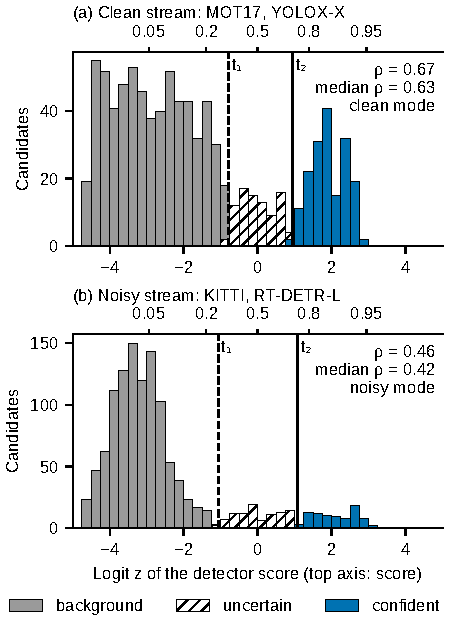
\includegraphics{Fig2.pdf}
\caption{What \scl{} sees just before its decision for frame 101: a histogram of the candidates
of the last 10 frames. Bottom axis: the logit of the detector score; top axis: the same position as
a score; height: the number of candidates. Dashed line: first split $t_1$; solid line: second split
$t_2$. Light bars: background (below $t_1$); hatched bars: uncertain (between the splits); dark
bars: confident (above $t_2$). $\rho$: the share of confident candidates in the foreground; the
median of $\rho$ decides the mode. (a) MOT17-02, published YOLOX-X detections, ByteTrack in its
official setting: $\rho=175/263=0.67$ and median $\rho=0.63\ge0.5$, so the stream is clean. (b)
KITTI 0001, RT-DETR-L, ByteTrack in its library setting: $\rho=83/182=0.46$ and median $\rho=0.42<0.5$,
so the stream is noisy. All values were recorded by the frozen \scl{} in the runs of
Sect.~\ref{sec:results}}
\label{fig:groups}
\end{figure}

\subsection{Median-Based Detection Stream Classification}\label{sec:regimes}
\emph{Step 2 in Fig.~\ref{fig:arch}. Input:} the values $\rho$ of all frames so far. \emph{Output:} the mode of frame $t$.

The mode describes the distribution of the scores, not whether a single detection is correct. The
stream is clean at frame $t$ if the median of all $\rho$ values so far is at least one half, a
majority rule, and noisy otherwise; before the first valid split it is cold. In
Fig.~\ref{fig:groups}a, the first frame has no past frames and is cold, and frames 2 to 101 give 100
values of $\rho$ whose median is 0.63, so frame 101 is clean; in Fig.~\ref{fig:groups}b the median of
the same 100 frames is 0.42, so it is noisy.

\emph{Mode stability and adaptation delay.} The whole-stream median trades speed for stability. A
short run of low scores, such as a few frames of blur or occlusion, cannot change the mode, so the
layer does not switch modes in the middle of a stream; during development this rule raised the
HOTA of ByteTrack and OC-SORT (Sect.~\ref{sec:steps}). The cost is a delay after a lasting change
of the detector within one stream: a stream that was clean for $N$ frames turns noisy only after
more than $N$ noisy frames, because only then do they form the majority of the $\rho$ values. Two
parts of the layer do not wait. The splits use only the last $W$ frames, so the groups, and in
the clean mode the thresholds of Step~3, follow a new score scale within $W$ frames, and the
recovery of Step~4 works in both modes; only the rescoring of the noisy mode waits for the mode. A
median over the last $K$ frames bounds the delay to about $K/2$ frames;
Sect.~\ref{sec:ablation} tests $K=100$ and $K=300$.

\subsection{Mode-Adaptive Detection Candidate Selection and Threshold Adjustment}\label{sec:choice}
\emph{Step 3 in Fig.~\ref{fig:arch}. Input:} $D_t$, the mode, $t_1$, $t_2$, the thresholds $a$, $b$, and the tracks
$\mathcal{T}_{t-1}$. \emph{Output:} the kept boxes, their scores, and the thresholds $a_t$, $b_t$.

\emph{Cold and clean modes.} The tracker keeps its own thresholds and scores, and only cross-class
duplicates are removed. In the clean mode, a threshold so high that it would reject the confident
group is lowered to the score $\sigma(t_2)$ at which that group begins:
\begin{equation}
a_t=\min\!\left(a,\sigma(t_2)\right),\qquad b_t=\min\!\left(b,\sigma(t_2)\right).
\label{eq:clean}
\end{equation}
In Fig.~\ref{fig:groups}a, $\sigma(t_2)=0.72$ is above both $a=0.6$ and $b=0.7$, so
$a_t=\min(0.6,0.72)=0.6$ and $b_t=\min(0.7,0.72)=0.7$: the published thresholds are kept. The clean
mode is thus a minimal intervention rather than a plain pass-through: the scores are
kept, and the output equals that of the host alone whenever the confident group lies above the
host's thresholds and no rescue applies, as for BoostTrack, ByteTrack at floor 0.1, and Hybrid-SORT
on MOT17 (Sect.~\ref{sec:results}). When the scores are halved, for example, no score is above 0.5,
and ByteTrack in its official setting ($a=0.6$, $b=0.7$) never starts a track; the splits move with
the halved scores, so $\sigma(t_2)$ falls below 0.5, Eq.~\eqref{eq:clean} lowers both thresholds to
it, and the confident candidates reach the tracker again.

\emph{Noisy mode.} Background candidates ($z<t_1$) are dropped. Each remaining score is
replaced by its mid-rank $u_i\in(0,1)$ among the scores of a remap memory: the share of the stored
scores that are lower than $s_i$, with equal scores counted half. The memory stores the scores
kept in the first frame and in every 10th frame, the last 20 of them (before the first sample the
current frame is used). The new score is
\begin{equation}
\tilde{s}_i=
\begin{cases}
0.5+0.5\,u_i, & z_i\ge t_2,\\
0.1+0.4\,u_i, & t_1\le z_i<t_2,
\end{cases}
\label{eq:remap}
\end{equation}
and both thresholds are set to $a_t=b_t=0.5$. For example, a confident candidate whose score is
higher than 80\% of the stored scores ($u_i=0.8$) gets $0.5+0.5\cdot0.8=0.9$, and an uncertain one
with $u_i=0.3$ gets $0.1+0.4\cdot0.3=0.22$. Confident candidates ($z\ge t_2$) then get scores above 0.5
and may start and continue tracks, and uncertain ones ($t_1\le z<t_2$) get scores below 0.5 and may
only continue tracks through a tracker's low-score step. A weaker
candidate that overlaps a stronger one with IoU above one half is removed, unless a different track
of the previous frame claims it, which keeps people who stand close together in a crowd.

\emph{Score remapping is not probability calibration.} Formal calibration learns, from labelled
data, a map from a score to the probability that the detection is correct \cite{kuppers2020detcalib}.
The remap of Eq.~\eqref{eq:remap} needs no labels and estimates no probability. It keeps the order
of the scores within each group and places the groups in fixed ranges, so that the tracker's own
thresholds read the decision of the layer: a score above 0.5 means ``may start a track'', a score
between 0.1 and 0.5 ``may only continue one''. A remapped score of 0.8 therefore says that the
candidate ranks high among recent confident candidates, not that it is correct with probability
0.8. Because only ranks are used, the remap itself is unchanged by any order-preserving change of
the detector's scores, whereas a learned calibration map would have to be learned again.

\subsection{Track-Guided Weak Detection Recovery}\label{sec:rescue}
\emph{Step 4 in Fig.~\ref{fig:arch}. Input:} the output of Step~3, the tracks $\mathcal{T}_{t-1}$, and $\ell$. \emph{Output:}
$K_t$, their scores, and $a_t$, $b_t$ for the tracker.

A track can be lost when its object gets low scores for a few frames, above all in single-stage
trackers, which have no low-score step. The rescue passes such a candidate, with its score raised
just above the lowest threshold of the frame ($\ell$ for a two-stage tracker, the lower of $a_t$
and $b_t$ for a single-stage one), when it is in the foreground (or, for a single-stage tracker,
when there is no background group), overlaps a track of the previous frame with IoU of at least
one half, no other usable candidate covers that track, and the tracker could not see it otherwise.
For example, for ByteTrack in its official setting (two-stage, $\ell=0.1$) a rescued candidate gets
$0.1+0.001=0.101$ and enters its low-score step; for OC-SORT in a noisy frame (single-stage,
$a_t=b_t=0.5$) it gets $0.501$. It thus gives single-stage trackers the continuation step they
lack. The rescue only makes the box
visible; the tracker itself still decides, with its own matching, whether and to which track it is
assigned.

\subsection{Camera Motion-Adaptive Matching Tolerance}\label{sec:motion}
\emph{Step 5 in Fig.~\ref{fig:arch}. Input:} the frames $I_{t-1}$, $I_t$ and the tolerance $m_0$. \emph{Output:} the tolerance
$m_t$ of frame $t$.

In noisy frames, the matching tolerance grows with camera motion, because fast motion moves boxes
far from their tracks; otherwise $m_t=m_0$. The motion $g_t$ is the shift between consecutive
grayscale frames at quarter resolution, found by phase correlation \cite{reddy1996phasecorr}, and
$r_t$ is its ratio to its median over the last 100 frames ($r_t=1$ during a warm-up of 5 frames or
if this median is zero):
\begin{equation}
m_t=\min\!\left(0.95,\;1-\frac{1-m_0}{\max(1,r_t)}\right).
\label{eq:motion}
\end{equation}
For example, with $m_0=0.8$ a match needs an IoU of at least $1-0.8=0.2$. If, in a noisy frame,
the camera moves twice as much as usual ($r_t=2$), then $m_t=\min(0.95,\,1-0.2/2)=0.9$, and a match
needs an IoU of only 0.1. The cap 0.95 keeps a smallest overlap of 0.05.

\subsection{SCL Integration with Existing Trackers}\label{sec:contract}
Table~\ref{tab:contracts} lists the contracts; each value is taken from the tracker's published
configuration, and none is fitted. For each tracker family, a small adapter links the layer to the
tracker block of Fig.~\ref{fig:arch}: it writes the layer's candidates, scores, thresholds, and
tolerance into the tracker's existing parameters before each update and then calls the tracker's
own update. The matching steps, motion model, track management, and any post-processing of the
authors run unchanged, so the host stays frozen: only the values of its thresholds are set for
each frame, and the rules are the same for every tracker.


\begin{table}[!tb]
\caption{The fixed values of \scl{}: each row gives one value, its setting, and where it comes from: a standard value of MOT evaluation, a common threshold, a definition, or a design choice made once at the start of development and never tuned. The same values are used for every tracker, detector, and dataset.}
\label{tab:constants}
\centering\footnotesize
\setlength{\tabcolsep}{3pt}
\begin{tabular}{@{}>{\raggedright\arraybackslash}p{19mm}>{\raggedright\arraybackslash}p{27mm}>{\raggedright\arraybackslash}p{25mm}@{}}
\toprule
Value & Setting & Source\\
\midrule
Window $W$ & 10 frames & design choice\\
Mode rule & clean if median $\rho\ge0.5$ & majority rule\\
Background check & $\rho=1$ if fewer below $t_1$ than above & rule: no background group\\
Noisy score ranges & $[0.5,1)$, $[0.1,0.5)$ & common thresholds\\
Noisy $a_t$, $b_t$ & 0.5 & common threshold\\
Remap memory & 20 frames, one every 10 & design choice\\
Duplicate, rescue IoU & 0.5 & MOT evaluation IoU\\
Rescued score & lowest threshold $+\,0.001$ & just above the threshold\\
Motion cue & phase correlation, quarter resolution & standard method \cite{reddy1996phasecorr}\\
Motion history & 100 frames, warm-up 5 & design choice\\
Tolerance cap & 0.95 & minimum overlap 0.05\\
\bottomrule
\end{tabular}
\end{table}

\subsection{Fixed SCL Parameters}\label{sec:constants}
Table~\ref{tab:constants} lists all values of \scl{}. They were fixed before the external
evaluation, are the same for every tracker, detector, and dataset, and none was chosen by searching
over a range of values. They come from standard values (the IoU of 0.5 of MOT evaluation and the
common thresholds 0.5 and 0.1), from definitions, and from design choices kept fixed in all
development stages. Algorithm~\ref{alg:layer} gives Steps 1--5 for one frame.

\begin{algorithm}[t]
\caption{\scl{} for frame $t$; the comments name the steps of Fig.~\ref{fig:arch}. The window
holds the logits of frames $t-W$ to $t-1$, so the decision for frame $t$ uses no future frame.}\label{alg:layer}
\begin{algorithmic}[1]
\Require candidates $D_t$, tracks $\mathcal{T}_{t-1}$, motion cue $g_t$, contract $(a,b,\ell,m_0)$, constants of Table~\ref{tab:constants}
\Ensure candidates $K_t$, scores $\tilde{s}$, thresholds $a_t,b_t$, tolerance $m_t$
\State $z_i\gets$ logit of $s_i$ for all $i$ \Comment{Eq.~\eqref{eq:logit}}
\If{no valid split exists} \Comment{e.g., first frame}
  \State mode $\gets$ cold; $(a_t,b_t)\gets(a,b)$
\Else
  \State $(t_1,t_2)\gets$ nested Otsu on the window \Comment{Step 1}
  \State $\rho_t\gets$ Eq.~\eqref{eq:rho} with the background check
  \State mode $\gets$ clean if $\mathrm{median}(\rho)\ge0.5$, else noisy \Comment{Step 2}
\EndIf
\If{mode is cold or clean} \Comment{Step 3}
  \State remove cross-class duplicates; keep raw scores
  \If{clean} set $(a_t,b_t)$ by Eq.~\eqref{eq:clean}
  \EndIf
\Else \Comment{noisy mode}
  \State remove duplicates with track context
  \State drop $z<t_1$; remap scores by Eq.~\eqref{eq:remap}
  \State $a_t\gets0.5$; $b_t\gets0.5$
\EndIf
\State rescue continuations (not cold) \Comment{Step 4}
\State $m_t\gets$ Eq.~\eqref{eq:motion} if noisy, else $m_0$ \Comment{Step 5}
\State pass $K_t$, $\tilde{s}$, $a_t$, $b_t$, $m_t$ to the tracker
\State add the logits left after duplicate removal to the window
\State add $g_t$ to the motion history
\State store the tracks of frame $t$ after the tracker update
\end{algorithmic}
\end{algorithm}
